\documentclass[a4paper,12pt]{article} % добавить leqno в [] для нумерации слева
\usepackage[a4paper,top=1.3cm,bottom=2cm,left=1.5cm,right=1.5cm,marginparwidth=0.75cm]{geometry}
%%% Работа с русским языком
\usepackage{cmap}					% поиск в PDF
\usepackage{mathtext} 				% русские буквы в фомулах
\usepackage[T2A]{fontenc}			% кодировка
\usepackage[utf8]{inputenc}			% кодировка исходного текста
\usepackage[english,russian]{babel}	% локализация и переносы

\usepackage{multirow}
\usepackage{graphicx}
\usepackage{mathtools}
\usepackage{wrapfig}
\usepackage{tabularx}
\usepackage{amssymb}
\usepackage{hyperref}
\usepackage[rgb]{xcolor}
\hypersetup{colorlinks=true,urlcolor=blue}
%% Шрифты
\usepackage{euscript}	 % Шрифт Евклид
\usepackage{amsmath}
\usepackage{mathtools}
%%% Заголовок
\author{Lokhmatov Arseniy}
\title{Лабораторная работа по общей физике}

\date{\today}
\begin{document}
\begin{titlepage}
    \newpage
    \begin{center}
    {\large МОСКОВСКИЙ ФИЗИКО-ТЕХНИЧЕСКИЙ ИНСТИТУТ (НАЦИОНАЛЬНЫЙ ИССЛЕДОВАТЕЛЬСКИЙ УНИВЕРСИТЕТ)}
    \vspace{1cm}

    {\largeФизтех-школа аэрокосмических технологий}
    \vspace{6em}
    \end{center}
    
    \vspace{1.2em}

    \begin{center}
    %\textsc{\textbf{}}
    \Large Лабораторная работа №4.3.2 \\
    Дифракция света на ультразвуковой волне в жидкости\\
    на установке с вертикальной щелью
    \linebreak
    \end{center}
    
    \vspace{11em}
    
    \begin{flushright}
                       {\large Работу выполнил\\
                       Лохматов Арсений Игоревич\\
                       Бегинин Тимофей Игоревич\\
                       Б03-303 }
    \end{flushright}

    \vspace{\fill}

    \begin{center}
        
\includegraphics[width=0.2\linewidth]{dasr.png}
    \end{center}

    \begin{center}
    Долгопрудный, 2025
    \end{center}

    \end{titlepage}

\section{Теоретическая часть}

\paragraph{Цель работы:} ознакомиться с методами получения и анализа поляризованного света.

\paragraph{Оборудование:} оптическая скамья, осветитель, светофильтры, конденсатор, щель, два длиннофокусных объектива, кювета с водой, кварцевый излучатель с микрометрическим винтом, генератор ульразвуковой частоты, частотометр, линза, отсчётное устройство, микроскоп.

\paragraph{Экспериментальная установка} для наблюдения дифракции света на УЗ-волных изображена на рисунке $\ref{img1}$.

\begin{figure}[h]
    \begin{center}
        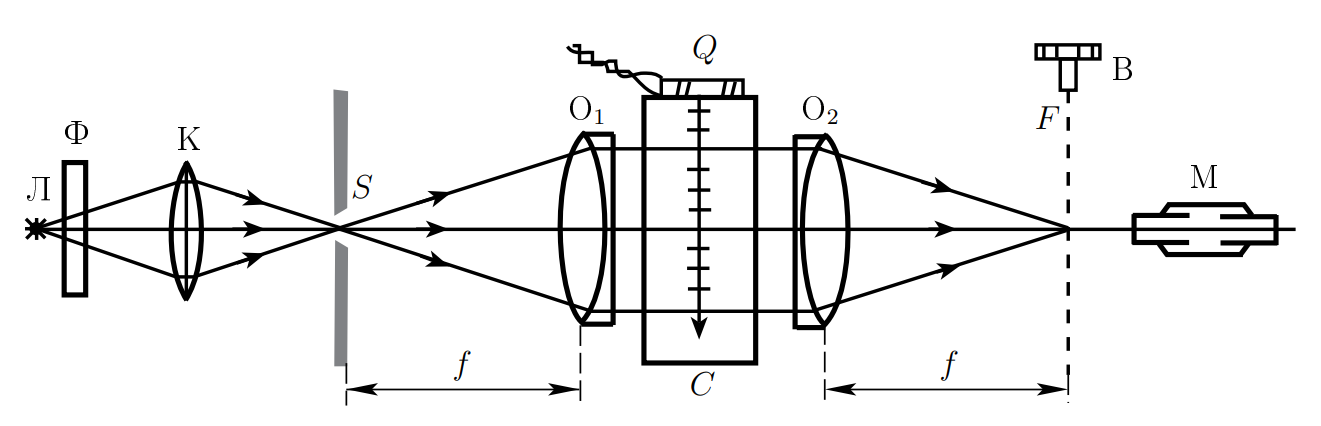
\includegraphics[width=16cm]{img1.png}
    \end{center}
    \caption{Схема наблюдения дифракции на акустической решётке}
    \label{img1}
\end{figure}

Источник света $\text{Л}$ через светофильтр $\text{Ф}$ и конденсор $\text{К}$ освещает щель $S$, которая расположена в фокусе объектива $O_1$. Выходящий из объектива параллельный пучок света проходит через кювету $C$ перпендикулярно направлению распространения УЗ-волн. Эти волны возбуждаются в жидкости пьезокварцевой пластинкой $Q$, прикреплённой к стенке кюветы. На кварцевую пластинку подаётся синусоидальное напряжения ультразвуковой частоты от генератора. В результате взаимодействия света с ультразвуковой волной в фокальной плоскости второго объектива $O_2$ образуется дифракционная картина, наблюдаемая при помощи микроскопа М. При этом обязательно применяют монохроматическое излучение (красный светофильтр).

\begin{wrapfigure}{r}{0.3\linewidth} 
    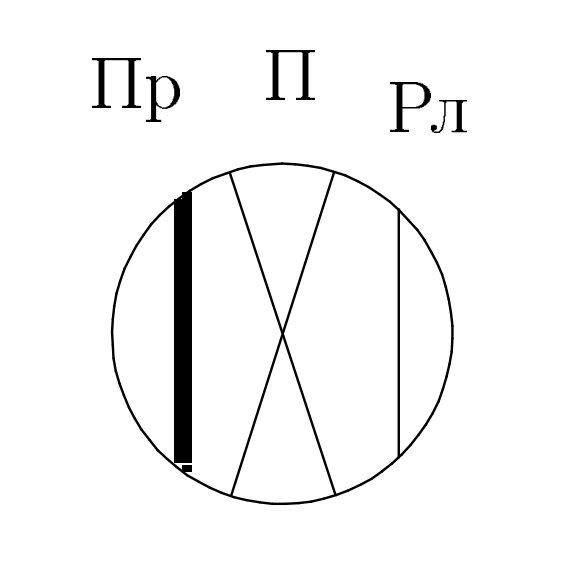
\includegraphics[width=\linewidth]{img2.png}
    \caption{Проволока $\text{Пр}$, перекрестие $\text{П}$ и реперная линия $\text{Рл}$ на стекле отсчётного устройства}
    \label{img2}
\end{wrapfigure}

Дифракционные полосы ориентированы вертикально. Расстояние между ними можно измерить с помощью специального отсчётного устройства с микрометрическим винтом $\text{В}$. Этот винт передвигает размещённые на стекле отсчётного устройства (рисунок $\ref{img2}$) тонкую реперную линию $\text{Рл}$, перекрестие $\text{П}$ и толстую проволоку $\text{Пр}$, которая используется в методе тёмного поля. Все измерительные линии должны быть расположены в плоскости $F$ резкого изображения щели.

Чёткость дифракционных полос зависит от ряда факторов, например, от ширины щели $S$, от её наклона по отношению к вертикали, от угла наклона кюветы к падающему лучу.

Длина $\Lambda$ ультразвуковой волны определяется формулой

\[ \Lambda\sin{\Theta_{m}}=m\lambda; \]

в силу малости углов $\Theta_{m}$ окончательное выражение может быть представлено в виде

\[ l_{m}=mf\frac{\lambda}{\Lambda}, \]

где $l_{m}$ -- измеренное на опыте линейное расстояние между $m-$м и нулевым максимумами, а $f$ -- фокусное расстояние объектива $O_2$.

Скорость $v$ распространения звука в воде можно рассчитать, если известна частота $\nu$ кварцевого излучателя:

\[ v=\Lambda\nu. \]

\paragraph{Наблюдение оптических неоднородностей, создаваемых ультразвуковыми волнами в жидкости методом тёмного поля.} Попробуем теперь получить видимое изображение фазовой акустической решётки. Для этого прежде всего необходимо получить в поле зрения микроскопа изображение задней плоскости (считая по ходу световых лучей) кюветы. Это достигается с помощью вспомогательной положительной линзы $O$, которую располагают на оптической скамье за фокальной плоскостью объектива $O_2$ (рисунок \ref{img3}).

Перемещая микроскоп вдоль оптической скамьи, фокусируют его на плоскость $P$, где расположено чёткое изображение $a'b'$ какого-либо предмета $ab$, вплотную прижвтого к стенке кюветы. Можно ли теперь увидеть в микроскоп акустическую решётку -- УЗ-волну? Ясно, что чисто фазовая решётка является невидимой, если, конечно, выполнено условие:

\[ m \ll \frac{\Lambda}{L}\sqrt{\frac{\lambda}{L}}. \]

\begin{figure}[h]
    \begin{center}
        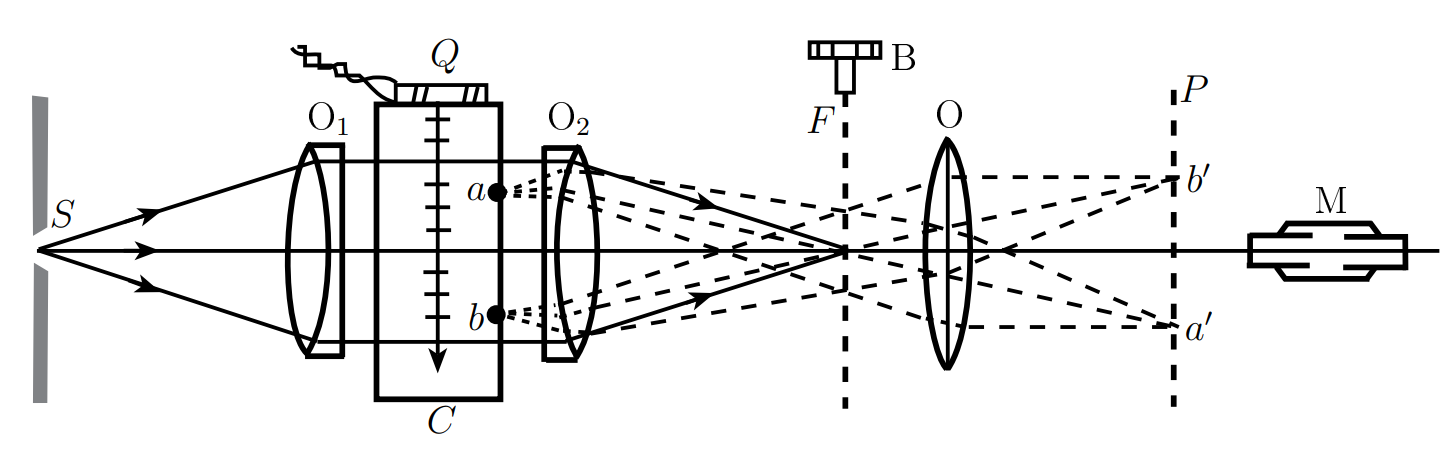
\includegraphics[width=16cm]{img3.png}
    \end{center}
    \caption{Наблюдение акустической решётки методом тёмного поля}
    \label{img3}
\end{figure}

Для наблюдения акустической решётки в работе используется $\text{метод тёмного поля}$, основанный на устранении центрального дифракционного максимума с помощью специального экрана (проволочки). В поле зрения микроскопа наблюдаются чередующиесясветлые и тёмные полосы, причём расстояние между тёмными полосами соответствует смещению в плоскости кюветы на $\Lambda/2$. Таким образом, наблюдается характерное для метода тёмного поля удвоения числа деталей рассматриваемой структуры.

\section{Практическая часть}

\subsection{Определение скорости ультразвука по дифракционной картине}

\begin{enumerate}
    \item Собрали установку согласно рисунку $\ref{img1}$. Для получения параллельного пучка щель $S$ должна быть установлена на фокусном расстоянии от главной плоскости объектива $O_1$. Объективы $O_1$ и $O_2$ одинаковы ($f=30\text{ см}$), поэтому ход лучей в правильно настроенной системе должен быть симметричным.
    \item Ярко осветили щель с помощью конденсора. Предварительную настройку вели с зелёным фильтром.
    \item Получили в поле зрения микроскопа систему дифракционных полос. Картина видна наиболее чётко, когда в кювете образуется стоячая УЗ-волна.
    \item Заменили зелёный фильтр красным. Изменяя ширину щели $S$, её наклон и положение конденсора, добились оптимальных условий наблюдения дифракционных полос.
    \item Заметили, что число дифракционных полос уменьшается при уменьшении мощности источника ультразвука.
    \item Снова получили чёткую дифракционную картину. Перемещая излучатель с помощью микрометрического винта, оценили на месте длину УЗ-волны как удвоенное расстояние между наиболее чёткими дифракционными картинами.

    \[ x_1 = (2.18\pm0.01)\text{ мм}, \text{ }x_2 = (2.88\pm0.01)\text{ мм} \Rightarrow \Delta x = |x_1-x_2|=(0.7\pm0.01)\text{ мм} \Rightarrow\]
    \[ \Rightarrow \Lambda=2\cdot\Delta x=(1.4\pm0.02)\text{ мм} \]

    Определили рабочую частоту по показанию частотометра: $\nu=1.1537\text{ МГц}$. По результатам измерений оценили скорость звука в воде, используя формулу:

    \[ v=\Lambda\nu \Rightarrow v = 1.4\cdot10^{-6}\cdot1.1537\cdot10^{6}=(1.615\pm0.023)\text{ }\frac{\text{км}}{\text{с}}. \]

    \item Для выбранной пяти частот в интервале от $1$ до $8\text{ МГц}$ определили положения $x_{m}$ нескольких дифракционных максимумов с помощью микрометрического винта отсчётного устройства. Положения максимумов мы отцентровали по нулевому. Результаты представлены в таблице $\ref{tab1}$.

    \begin{table}[h]
        \centering
        \begin{tabular}{|c|c|}
        \hline
            \multicolumn{2}{|c|}{$\nu_1=1.154\text{ МГц}$} \\ \hline
        \hline
    	$m$ & $x_m, \text{ мкм}$ \\ \hline
    	-3 & -472 \\ \hline
    	-2 & -304 \\ \hline
    	-1 & -156 \\ \hline
    	0 & 0 \\ \hline
    	1 & 160 \\ \hline
    	2 & 312 \\ \hline
            3 & 476 \\ \hline
        \end{tabular}
        \begin{tabular}{|c|c|}
        \hline
            \multicolumn{2}{|c|}{$\nu_2=1.829\text{ МГц}$} \\ \hline
        \hline
    	$m$ & $x_m, \text{ мкм}$ \\ \hline
    	-2 & -480 \\ \hline
    	-1 & -244 \\ \hline
    	0 & 0 \\ \hline
    	1 & 224 \\ \hline
    	2 & 492 \\ \hline
        \end{tabular}
        \begin{tabular}{|c|c|}
        \hline
            \multicolumn{2}{|c|}{$\nu_3=3.468\text{ МГц}$} \\ \hline
        \hline
    	$m$ & $x_m, \text{ мкм}$ \\ \hline
    	-1 & -436 \\ \hline
    	0 & 0 \\ \hline
    	1 & 496 \\ \hline
        \end{tabular}
        \begin{tabular}{|c|c|}
        \hline
            \multicolumn{2}{|c|}{$\nu_4=3.958\text{ МГц}$} \\ \hline
        \hline
    	$m$ & $x_m, \text{ мкм}$ \\ \hline
    	-2 & -1036 \\ \hline
    	-1 & -516 \\ \hline
    	0 & 0 \\ \hline
    	1 & 592 \\ \hline
    	2 & 1048 \\ \hline
        \end{tabular}
        \begin{tabular}{|c|c|}
        \hline
            \multicolumn{2}{|c|}{$\nu_5=6.295\text{ МГц}$} \\ \hline
        \hline
    	$m$ & $x_m, \text{ мкм}$ \\ \hline
    	-1 & -840 \\ \hline
    	0 & 0 \\ \hline
    	1 & 836 \\ \hline
        \end{tabular}
    \caption{Результаты измерений для различных частот ультразвуковых волн}
    \label{tab1}
    \end{table}
    \item Записали фокусное расстояние объектива $O_2$: $f=30\text{ см}$; и полосу пропускания светофильтра: $(6400\pm200)\text{ А}$.
    \item Для каждой частоты построили график зависимости координаты $x_m$ от порядка $m$ и по наклону прямой определили расстояние между соседними полосами $l_{m}/m=\Delta x_{m}/\Delta m$.  Рассчитали длину $\Lambda$ УЗ-волны и скорость ультразвука в воде. Оценили погрешность эксперимента.
\end{enumerate}

\newpage
\paragraph{$\nu_1=1.154\text{ МГц}$:} график представлен на рисунке $\ref{img4}$.

\begin{figure}[h]
    \begin{center}
        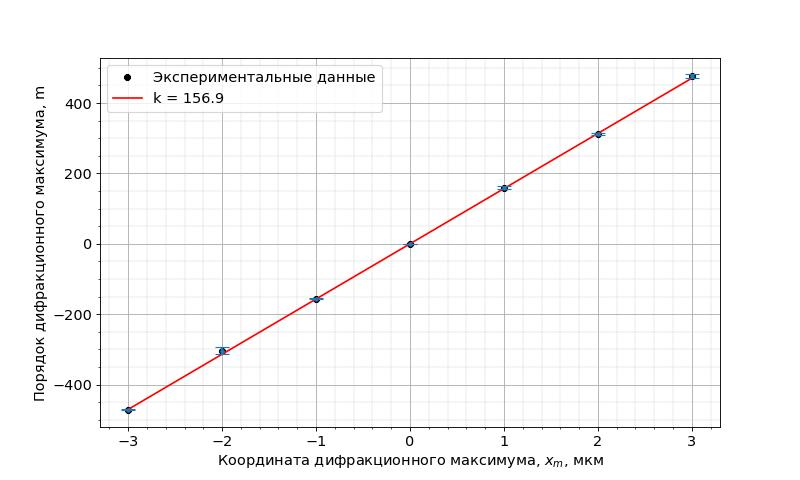
\includegraphics[width=16cm]{image1.jpg}
    \end{center}
    \caption{График зависимости функции $x_m=F(m)$ для частоты $\nu_1=1.154\text{ МГц}$}
    \label{img4}
\end{figure}

\[ k = \frac{\Delta x_{m}}{m} = (156.9\pm0.9)\text{ }\frac{1}{\text{мкм}} \Rightarrow \frac{l_{m}}{m} = (156.9\pm0.9)\text{ }\frac{1}{\text{мкм}} \]
\[ l_{m}=mf\frac{\lambda}{\Lambda} \Rightarrow \Lambda = f\lambda\frac{m}{l_{m}} \Rightarrow  \]
\[ \Rightarrow \Lambda_1 = 30\cdot10^{-2}\cdot6400\cdot10^{-10}\cdot\frac{1}{156.9}\cdot10^{6}=1223.7\cdot10^{-6}\text{ м}. \]
\[ \sigma_{\Lambda} = \Lambda\sqrt{\Big(\frac{\sigma_{l_{m}/m}}{l_{m}/m}\Big)^2+ \Big(\frac{\sigma_{\lambda}}{\lambda}\Big)^2} \Rightarrow \sigma_{\Lambda_1} = 1223.7\cdot10^{-6}\cdot\sqrt{\Big(\frac{0.9}{156.9}\Big)^2+\Big(\frac{200}{6400}\Big)^2} = 38.9\cdot10^{-6}\text{ м}. \]

\centering\boxed{\Lambda_1=(1223.7\pm38.9)\cdot10^{-6}\text{ м}\text{ }(\varepsilon=3.2\%).}

\[ v=\Lambda\nu \Rightarrow v_1=1223.7\cdot10^{-6}\cdot1.154\cdot10^{6}=1412.2\text{ }\frac{\text{м}}{\text{с}}. \]
\[ \sigma_{v} = v\sqrt{\Big(\frac{\sigma_{\Lambda}}{\Lambda}\Big)^2} \Rightarrow \sigma_{v_1} = 1412.2\cdot\frac{38.9\cdot10^{-6}}{1223.7\cdot10^{-6}} = 44.9\text{ }\frac{\text{м}}{\text{с}}. \]

\boxed{v_{1}=(1412.2\pm44.9)\text{ }\frac{\text{м}}{\text{с}}\text{ }(\varepsilon=3.2\%).}

\newpage

\raggedright\paragraph{$\nu_2=1.829\text{ МГц}$:} график представлен на рисунке $\ref{img5}$.

\begin{figure}[h]
    \begin{center}
        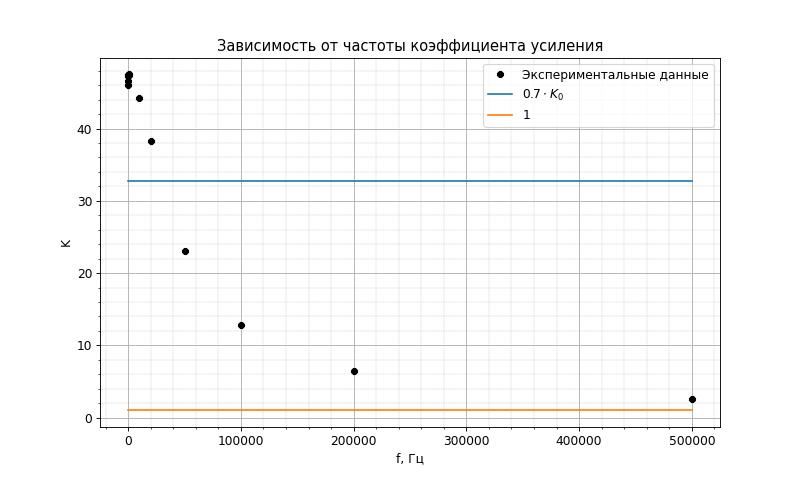
\includegraphics[width=16cm]{image2.jpg}
    \end{center}
    \caption{График зависимости функции $x_m=F(m)$ для частоты $\nu_2=1.829\text{ МГц}$}
    \label{img5}
\end{figure}

\[ k = \frac{\Delta x_{m}}{m} = (241.2\pm3.2)\text{ }\frac{1}{\text{мкм}} \Rightarrow \frac{l_{m}}{m} = (241.2\pm3.2)\text{ }\frac{1}{\text{мкм}} \]
\[ l_{m}=mf\frac{\lambda}{\Lambda} \Rightarrow \Lambda = f\lambda\frac{m}{l_{m}} \Rightarrow  \]
\[ \Rightarrow \Lambda_2 = 30\cdot10^{-2}\cdot6400\cdot10^{-10}\cdot\frac{1}{241.2}\cdot10^{6}=796.1\cdot10^{-6}\text{ м}. \]
\[ \sigma_{\Lambda} = \Lambda\sqrt{\Big(\frac{\sigma_{l_{m}/m}}{l_{m}/m}\Big)^2+ \Big(\frac{\sigma_{\lambda}}{\lambda}\Big)^2} \Rightarrow \sigma_{\Lambda_2} = 796.1\cdot10^{-6}\cdot\sqrt{\Big(\frac{3.2}{241.2}\Big)^2+\Big(\frac{200}{6400}\Big)^2} = 27.1\cdot10^{-6}\text{ м}. \]

\centering\boxed{\Lambda_2=(796.1\pm27.1)\cdot10^{-6}\text{ м}\text{ }(\varepsilon=3.4\%).}

\[ v=\Lambda\nu \Rightarrow v_2=796.1\cdot10^{-6}\cdot1.829\cdot10^{6}=1456.1\text{ }\frac{\text{м}}{\text{с}}. \]
\[ \sigma_{v} = v\sqrt{\Big(\frac{\sigma_{\Lambda}}{\Lambda}\Big)^2} \Rightarrow \sigma_{v_2} = 1456.1\cdot\frac{27.1\cdot10^{-6}}{796.1\cdot10^{-6}} = 49.6\text{ }\frac{\text{м}}{\text{с}}. \]

\centering\boxed{v_{2}=(1456.1\pm49.6)\text{ }\frac{\text{м}}{\text{с}}\text{ }(\varepsilon=3.4\%).}

\newpage

\raggedright\paragraph{$\nu_3=3.468\text{ МГц}$:} график представлен на рисунке $\ref{img6}$.

\begin{figure}[h]
    \begin{center}
        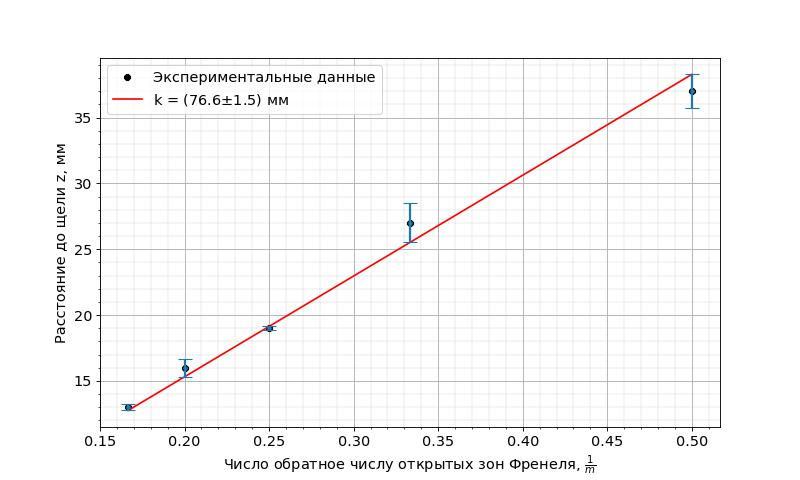
\includegraphics[width=16cm]{image3.jpg}
    \end{center}
    \caption{График зависимости функции $x_m=F(m)$ для частоты $\nu_3=3.468\text{ МГц}$}
    \label{img6}
\end{figure}

\[ k = \frac{\Delta x_{m}}{m} = (466.0\pm21.2)\text{ }\frac{1}{\text{мкм}} \Rightarrow \frac{l_{m}}{m} = (466.0\pm21.2)\text{ }\frac{1}{\text{мкм}} \]
\[ l_{m}=mf\frac{\lambda}{\Lambda} \Rightarrow \Lambda = f\lambda\frac{m}{l_{m}} \Rightarrow  \]
\[ \Rightarrow \Lambda_3 = 30\cdot10^{-2}\cdot6400\cdot10^{-10}\cdot\frac{1}{466.0}\cdot10^{6}=412.0\cdot10^{-6}\text{ м}. \]
\[ \sigma_{\Lambda} = \Lambda\sqrt{\Big(\frac{\sigma_{l_{m}/m}}{l_{m}/m}\Big)^2+ \Big(\frac{\sigma_{\lambda}}{\lambda}\Big)^2} \Rightarrow \sigma_{\Lambda_3} = 412.0\cdot10^{-6}\cdot\sqrt{\Big(\frac{21.2}{466.0}\Big)^2+\Big(\frac{200}{6400}\Big)^2} = 22.7\cdot10^{-6}\text{ м}. \]

\centering\boxed{\Lambda_3=(412.0\pm22.7)\cdot10^{-6}\text{ м}\text{ }(\varepsilon=5.5\%).}

\[ v=\Lambda\nu \Rightarrow v_2=412.0\cdot10^{-6}\cdot3.468\cdot10^{6}=1428.8\text{ }\frac{\text{м}}{\text{с}}. \]
\[ \sigma_{v} = v\sqrt{\Big(\frac{\sigma_{\Lambda}}{\Lambda}\Big)^2} \Rightarrow \sigma_{v_3} = 1428.8\cdot\frac{22.7\cdot10^{-6}}{412.0\cdot10^{-6}} = 78.7\text{ }\frac{\text{м}}{\text{с}}. \]

\centering\boxed{v_{3}=(1428.8\pm78.7)\text{ }\frac{\text{м}}{\text{с}}\text{ }(\varepsilon=5.5\%).}

\newpage

\raggedright\paragraph{$\nu_4=3.958\text{ МГц}$:} график представлен на рисунке $\ref{img7}$.

\begin{figure}[h]
    \begin{center}
        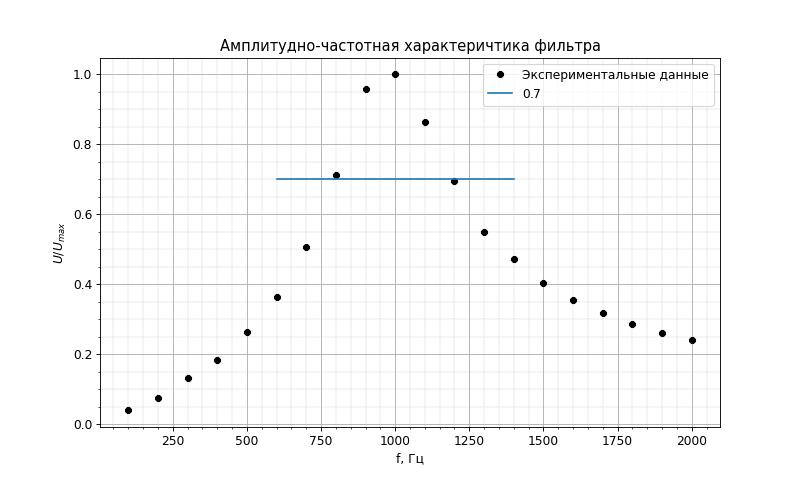
\includegraphics[width=16cm]{image4.jpg}
    \end{center}
    \caption{График зависимости функции $x_m=F(m)$ для частоты $\nu_4=3.958\text{ МГц}$}
    \label{img7}
\end{figure}

\[ k = \frac{\Delta x_{m}}{m} = (527.6\pm10.8)\text{ }\frac{1}{\text{мкм}} \Rightarrow \frac{l_{m}}{m} = (527.6\pm10.8)\text{ }\frac{1}{\text{мкм}} \]
\[ l_{m}=mf\frac{\lambda}{\Lambda} \Rightarrow \Lambda = f\lambda\frac{m}{l_{m}} \Rightarrow  \]
\[ \Rightarrow \Lambda_4 = 30\cdot10^{-2}\cdot6400\cdot10^{-10}\cdot\frac{1}{527.6}\cdot10^{6}=363.9\cdot10^{-6}\text{ м}. \]
\[ \sigma_{\Lambda} = \Lambda\sqrt{\Big(\frac{\sigma_{l_{m}/m}}{l_{m}/m}\Big)^2+ \Big(\frac{\sigma_{\lambda}}{\lambda}\Big)^2} \Rightarrow \sigma_{\Lambda_4} = 363.9\cdot10^{-6}\cdot\sqrt{\Big(\frac{10.8}{527.6}\Big)^2+\Big(\frac{200}{6400}\Big)^2} = 13.6\cdot10^{-6}\text{ м}. \]

\centering\boxed{\Lambda_4=(363.9\pm13.6)\cdot10^{-6}\text{ м}\text{ }(\varepsilon=3.7\%).}

\[ v=\Lambda\nu \Rightarrow v_4=363.9\cdot10^{-6}\cdot3.958\cdot10^{6}=1440.3\text{ }\frac{\text{м}}{\text{с}}. \]
\[ \sigma_{v} = v\sqrt{\Big(\frac{\sigma_{\Lambda}}{\Lambda}\Big)^2} \Rightarrow \sigma_{v_4} = 1440.3\cdot\frac{13.6\cdot10^{-6}}{363.9\cdot10^{-6}} = 53.8\text{ }\frac{\text{м}}{\text{с}}. \]

\centering\boxed{v_{4}=(1440.3\pm53.8)\text{ }\frac{\text{м}}{\text{с}}\text{ }(\varepsilon=3.7\%).}

\newpage

\raggedright\paragraph{$\nu_5=6.295\text{ МГц}$:} график представлен на рисунке $\ref{img8}$.

\begin{figure}[h]
    \begin{center}
        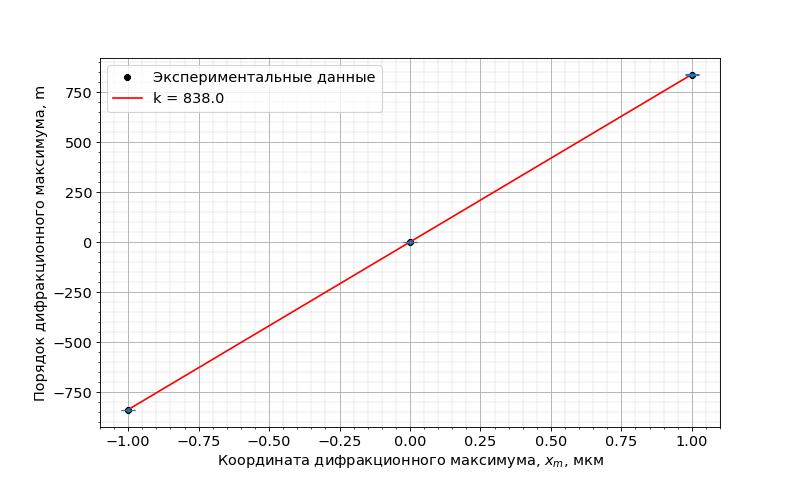
\includegraphics[width=16cm]{image5.jpg}
    \end{center}
    \caption{График зависимости функции $x_m=F(m)$ для частоты $\nu_5=6.295\text{ МГц}$}
    \label{img8}
\end{figure}

\[ k = \frac{\Delta x_{m}}{m} = (838.0\pm1.4)\text{ }\frac{1}{\text{мкм}} \Rightarrow \frac{l_{m}}{m} = (838.0\pm1.4)\text{ }\frac{1}{\text{мкм}} \]
\[ l_{m}=mf\frac{\lambda}{\Lambda} \Rightarrow \Lambda = f\lambda\frac{m}{l_{m}} \Rightarrow  \]
\[ \Rightarrow \Lambda_5 = 30\cdot10^{-2}\cdot6400\cdot10^{-10}\cdot\frac{1}{838.0}\cdot10^{6}=229.1\cdot10^{-6}\text{ м}. \]
\[ \sigma_{\Lambda} = \Lambda\sqrt{\Big(\frac{\sigma_{l_{m}/m}}{l_{m}/m}\Big)^2+ \Big(\frac{\sigma_{\lambda}}{\lambda}\Big)^2} \Rightarrow \sigma_{\Lambda_5} = 229.1\cdot10^{-6}\cdot\sqrt{\Big(\frac{1.4}{838.0}\Big)^2+\Big(\frac{200}{6400}\Big)^2} = 7.2\cdot10^{-6}\text{ м}. \]

\centering\boxed{\Lambda_5=(229.1\pm7.2)\cdot10^{-6}\text{ м}\text{ }(\varepsilon=3.1\%).}

\[ v=\Lambda\nu \Rightarrow v_5=229.1\cdot10^{-6}\cdot6.295\cdot10^{6}=1442.2\text{ }\frac{\text{м}}{\text{с}}. \]
\[ \sigma_{v} = v\sqrt{\Big(\frac{\sigma_{\Lambda}}{\Lambda}\Big)^2} \Rightarrow \sigma_{v_5} = 1442.2\cdot\frac{7.2\cdot10^{-6}}{229.1\cdot10^{-6}} = 45.3\text{ }\frac{\text{м}}{\text{с}}. \]

\centering\boxed{v_{5}=(1442.2\pm45.3)\text{ }\frac{\text{м}}{\text{с}}\text{ }(\varepsilon=3.1\%).}

\newpage

\raggedright\subsection{Определение скорости ультразвука методом тёмного поля}

\begin{enumerate}
    \item Выключили генератор для того, чтобы в микроспоп было видно только изображение входнйо щели. Не смещая микроскоп, ввели микрометрическим винтом в поле зрения микроскопа вертикальную нить так, чтобы резкое изображение нити совпадало с резким изображением щели.
    
    Не меняя положения отсчётного устройства, отодвинули микроскоп и поставили дополнительную линзу сразу за отсчётным микроскопом согласно рисунку $\ref{img3}$.
    \item Опустили в воду пластинку с миллиметровыми делениями и прижали её к задней стенке кюветы. Открыли пошире входную щель. Передвигая микроскоп, сфокусировали его на изображении линейки.
    \item Для данного положения микроскопа определили цену деления окулярной шкалы в условиях опыта. Получили, что 18 штрихов окулярной шкалы соответствует 1-му делению линейки. Значит, цена деления окулярной шкалы составляет $l_0=\frac{1}{18}\text{ мм}$.
    \item Убрали пластинку из кюветы и уменьши ширину входной щели. Включили генератор. В микроскоп наблюдали звуковую решётку.
    \item Определили длину УЗ-волны в воде. Для этого для 4-ёх частот с помощью окулярной шкалы измерили расстояние между самыми дальними из хорошо видимых в поле зрения тёмных полос и посчитали число промежутков между ними. Так же определили частоту с помощью частотометра. Результаты измерений представлены в таблице $\ref{tab2}$.

    \begin{table}[h]
        \centering
        \begin{tabular}{|c|c|c|c|c|}
        \hline
    	$N$ & $\nu, \text{ МГц}$ & $n_{\text{штрихов}}$ & $l\cdot10^{-6}, \text{ м}$ & $m_{\text{миним}}$ \\ \hline
    	1 & 1.196 & 43 & 2389 & 4 \\ \hline
    	2 & 1.558 & 41 & 2278 & 5 \\ \hline
    	3 & 1.835 & 65 & 3611 & 9 \\ \hline
    	4 & 4.009 & 20 & 1111 & 6 \\ \hline
        \end{tabular}
    \caption{Результаты измерений для различных частот ультразвуковых волн в опыте с применением тёмного поля}
    \label{tab2}
    \end{table}
\end{enumerate}

\paragraph{$\nu_1=1.196\text{ МГц}$:}

\[ \frac{\Lambda}{2} = \frac{l}{m} \Rightarrow \Lambda=\frac{2l}{m} \Rightarrow \Lambda_1=\frac{2\cdot2389\cdot10^{-6}}{4} = 1194.5\cdot10^{-6}\text{ м}; \]
\[ v=\Lambda\nu \Rightarrow v_1= 1194.5\cdot10^{-6}\cdot1.196\cdot10^{6}=1428.6\text{ }\frac{\text{м}}{\text{с}}. \]

\paragraph{$\nu_2=1.556\text{ МГц}$:}

\[ \frac{\Lambda}{2} = \frac{l}{m} \Rightarrow \Lambda=\frac{2l}{m} \Rightarrow \Lambda_2=\frac{2\cdot2278\cdot10^{-6}}{5} = 911.2\cdot10^{-6}\text{ м}; \]
\[ v=\Lambda\nu \Rightarrow v_2= 911.2\cdot10^{-6}\cdot1.556\cdot10^{6}=1417.8\text{ }\frac{\text{м}}{\text{с}}. \]

\paragraph{$\nu_3=1.835\text{ МГц}$:}

\[ \frac{\Lambda}{2} = \frac{l}{m} \Rightarrow \Lambda=\frac{2l}{m} \Rightarrow \Lambda_3=\frac{2\cdot3611\cdot10^{-6}}{9} = 802.4\cdot10^{-6}\text{ м}; \]
\[ v=\Lambda\nu \Rightarrow v_3= 802.4\cdot10^{-6}\cdot1.835\cdot10^{6}=1472.5\text{ }\frac{\text{м}}{\text{с}}. \]

\paragraph{$\nu_4=4.009\text{ МГц}$:}

\[ \frac{\Lambda}{2} = \frac{l}{m} \Rightarrow \Lambda=\frac{2l}{m} \Rightarrow \Lambda_4=\frac{2\cdot1111\cdot10^{-6}}{6} = 370.3\cdot10^{-6}\text{ м}; \]
\[ v=\Lambda\nu \Rightarrow v_4= 370.3\cdot10^{-6}\cdot4.009\cdot10^{6}=1484.7\text{ }\frac{\text{м}}{\text{с}}. \]

\section{Подведение итогов и выводы}

В ходе данной работы мы исследовали дифракцию света на ультразвуковой волне в жидкости на установке с вертикальной щелью.
В результате исследования, мы определили скорость ультразвука по дифракционной картине. Результат представлены в свобной таблице $\ref{tab3}$.

\begin{table}[h]
    \centering
    \begin{tabular}{|c|c|c|c|c|c|}
    \hline
    $N$ & $\nu, \text{ МГц}$ & $\Lambda\cdot10^{-6}, \text{ м}$ & $\sigma_{\Lambda}\cdot10^{-6}, \text{ м}$ & $v, \text{ }\frac{\text{м}}{\text{с}}$ & $\sigma_{v}, \text{ }\frac{\text{м}}{\text{с}}$ \\ \hline
    1 & 1.154 & 1223.7 & 38.9 & 1412.2 & 44.9 \\ \hline
    2 & 1.829 & 796.1 & 27.1 & 1456.1 & 49.6 \\ \hline
    3 & 3.468 & 412.0 & 22.7 & 1428.8 & 78.8 \\ \hline
    4 & 3.958 & 363.9 & 13.6 & 1440.3 & 53.8 \\ \hline
    5 & 6.295 & 229.1 & 7.2 & 1442.2 & 45.3 \\ \hline
    \end{tabular}
\caption{Свобная таблица}
\label{tab3}
\end{table}

По табличным данным скорость распространения ультразвуковых волн в воде составляет $v^{table}\approx1500\text{ }\frac{\text{м}}{\text{с}}$. Полученные значения с учётом погрешности очень близки к табличному, что говорит о точности метода определения скорости ультразвуковых волн.

Вторым экспериментов в данной лабораторной работе было определение скорости ультразвука методом тёмного поля. Несмотря на то, что звуковая решётка в ходе выполнения получилась не очень чёткой, мы смогли снять измерения и рассчитать скорость ультразвука. Результаты представлены в таблице $\ref{tab4}$.

\begin{table}[h]
    \centering
    \begin{tabular}{|c|c|c|c|}
    \hline
    $N$ & $\nu, \text{ МГц}$ & $\Lambda\cdot10^{-6}, \text{ м}$ & $v, \text{ }\frac{\text{м}}{\text{с}}$ \\ \hline
    1 & 1.196 & 1194.5 & 1428.6 \\ \hline
    2 & 1.556 & 911.2 & 1417.8 \\ \hline
    3 & 1.835 & 802.4 & 1472.5 \\ \hline
    4 & 4.009 & 370.3 & 1484.7 \\ \hline
    \end{tabular}
\caption{Свобная таблица при измерении методом тёмного поля}
\label{tab4}
\end{table}

И в этом случае результаты с цчётом погрешности так же соответствуют табличному значению.

\end{document}
